% Copyright 2004 by Till Tantau <tantau@users.sourceforge.net>.
%
% In principle, this file can be redistributed and/or modified under
% the terms of the GNU Public License, version 2.
%
% However, this file is supposed to be a template to be modified
% for your own needs. For this reason, if you use this file as a
% template and not specifically distribute it as part of a another
% package/program, I grant the extra permission to freely copy and
% modify this file as you see fit and even to delete this copyright
% notice. 

%\documentclass{beamer}
\documentclass[aspectratio=169]{beamer}
\usepackage[utf8]{inputenc}
\usepackage[spanish]{babel}	



% There are many different themes available for Beamer. A comprehensive
% list with examples is given here:
% http://deic.uab.es/~iblanes/beamer_gallery/index_by_theme.html
% You can uncomment the themes below if you would like to use a different
% one:
%\usetheme{AnnArbor}
%\usetheme{Antibes}
%\usetheme{Bergen}
%\usetheme{Berkeley}
%\usetheme{Berlin}
%\usetheme{Boadilla}
%\usetheme{boxes}
%\usetheme{CambridgeUS}
%\usetheme{Copenhagen}
%\usetheme{Darmstadt}
%\usetheme{default}
%\usetheme{Frankfurt}
\usetheme{Goettingen}
%\usetheme{Hannover}
%\usetheme{Ilmenau}
%\usetheme{JuanLesPins}
%\usetheme{Luebeck}
%\usetheme{Madrid}
%\usetheme{Malmoe}
%\usetheme{Marburg}
%\usetheme{Montpellier}
%\usetheme{PaloAlto}
%\usetheme{Pittsburgh}
%\usetheme{Rochester}
%\usetheme{Singapore}
%\usetheme{Szeged}
%\usetheme{Warsaw}

\title{Extracción de Embocadura en Aliento/Arrugas}

% A subtitle is optional and this may be deleted
\subtitle{Procesamiento Digital de Señales de Audio - Curso 2016}

\author{Juan Braga}%\inst{1}}
% - Give the names in the same order as the appear in the paper.
% - Use the \inst{?} command only if the authors have different
%   affiliation.

\institute[IIE-FING-UDELAR] % (optional, but mostly needed)
{
  %\inst{1}%
  Instituto de Ingeniería Eléctrica (IIE)\\
  Facultad de Ingeniería (FING)\\
  Universidad de la República (UDELAR)}
% - Use the \inst command only if there are several affiliations.
% - Keep it simple, no one is interested in your street address.

\date{Diciembre 2016}
% - Either use conference name or its abbreviation.
% - Not really informative to the audience, more for people (including
%   yourself) who are reading the slides online

\subject{Procesamiento Digital de Señales de Audio - Curso 2016}
% This is only inserted into the PDF information catalog. Can be left
% out. 

% If you have a file called "university-logo-filename.xxx", where xxx
% is a graphic format that can be processed by latex or pdflatex,
% resp., then you can add a logo as follows:

% \pgfdeclareimage[height=0.5cm]{university-logo}{university-logo-filename}
% \logo{\pgfuseimage{university-logo}}

% Delete this, if you do not want the table of contents to pop up at
% the beginning of each subsection:
%\AtBeginSubsection[]
{%
 % \begin{frame}<beamer>{Outline}
 %   \tableofcontents[currentsection,currentsubsection]
 % \end{frame}
}%

% Let's get started
\begin{document}

\begin{frame}
  \titlepage
\end{frame}

\begin{frame}{Agenda}
  \tableofcontents
  % You might wish to add the option [pausesections]
\end{frame}

% Section and subsections will appear in the presentation overview
% and table of contents.
\section{Introducción}

\begin{frame}{Introducción}{Flauta Traversa}
  \begin{itemize}
  \item {
    Flauta Traversa perteneciente a la familia de las \textit{Maderas}
  }
  \item {
    Exitación periódica de la columna de aire generada por turbulencia de la colisión del flujo de aire contra el bisel de la embocadura.
  }
    \item {
    Altura definida por las llaves del instrumento.
  }
  \end{itemize}
\end{frame}

\begin{frame}{Introducción}{Técnicas Extendidas}
  \begin{itemize}
  \item {
    Exploración de nuevas sonoridades.
  }
  \item {
    Extensión de los límites naturales del instrumento.
  }
    \item {
    Técnicas reproducibles y bien definidas, generan que los instrumentistas tengan que expandir sus hablidades con el instrumento.
  }
  \end{itemize}
\end{frame}

\begin{frame}{Introducción}{Extracción de contenido músical (MIR por su sigla en inglés)}
  \begin{itemize}
  \item {
    Las alturas y duraciones ya no definen el material sonoro.
  }
  \item {
    El repertorio contemporáneo define una área del MIR desafiante y de espectro más amplio.
  }
    \item {
   	Hay lugar a contribuciones científicas mediante el acercamiento al material sonoro exótico.
  }
  \end{itemize}
\end{frame}

\subsection{Embocadura}

% You can reveal the parts of a slide one at a time
% with the \pause command:
\begin{frame}{Embocadura}
  \begin{itemize}
  \item {
    Refiere al aparato de producción de la exitación de la columna de aire, en conjunto a la técnica de soplido.}
  \item {   
    Es determinante del material sonoro ejecutado, siendo perceptible de forma auditivia a través de cambios en la Dinámica, Altura y Timbre.
  }
  % You can also specify when the content should appear
  % by using <n->:
  \item {
    Parámetros físicos que determinan la embocadura:
    \begin{itemize}
    	\item Ángulo de la Flauta.
     	\item Apertura de los labios.
     	\item Posición de los labios.
     	\item Presión de Aire.
    \end{itemize}
  }

  \end{itemize}
\end{frame}

\subsection{Aliento/Arrugas de Marcelo Toledo}

% You can reveal the parts of a slide one at a time
% with the \pause command:
\begin{frame}{Aliento/Arrugas de Marcelo Toledo}{Sobre la pieza}
  \begin{itemize}
  \item {
    Obra para Flauta Traversa solista, compuesta por el argentino Marcelo Toledo.
    %\pause % The slide will pause after showing the first item
  }
  \item {   
    Emplea técnicas extendidas como recurso compositivo:
    \begin{itemize}
    	\item \textit{Flutter Tonguing} - Aleteo de lengüa.
     	\item \textit{Tongue Noises} - Ruidos con la lengüa.
     	\item \textit{Percussive Sounds} - Llaveo.
     	\item \textit{Microtonal Inflections} - Inflecciones microtonales.
     	\item \textit{Multiphonics} - Sonidos multifónicos (cantar y tocar a la vez).
    \end{itemize}
  }
  % You can also specify when the content should appear
  % by using <n->:
  \item {
    Además emplea como recurso expresivo cambios en la embocadura a lo largo de la pieza. Detallando en la partitura la embocadura correspondiente .
  }
  \item {   
    Tres tipos de embocadura:
    \begin{itemize}
    	\item \textit{Blow Hole Covert} - Embocadura normal o tradicional.
     	\item \textit{Normal Embouchure} - Agüjero cubierto.
     	\item \textit{Breathy Embouchure} - Embocadura con aire.
    \end{itemize}
  }
  \end{itemize}
\end{frame}
 
\begin{frame}{Aliento/Arrugas de Marcelo Toledo}{Notación}
\begin{figure}[H]
\begin{center}
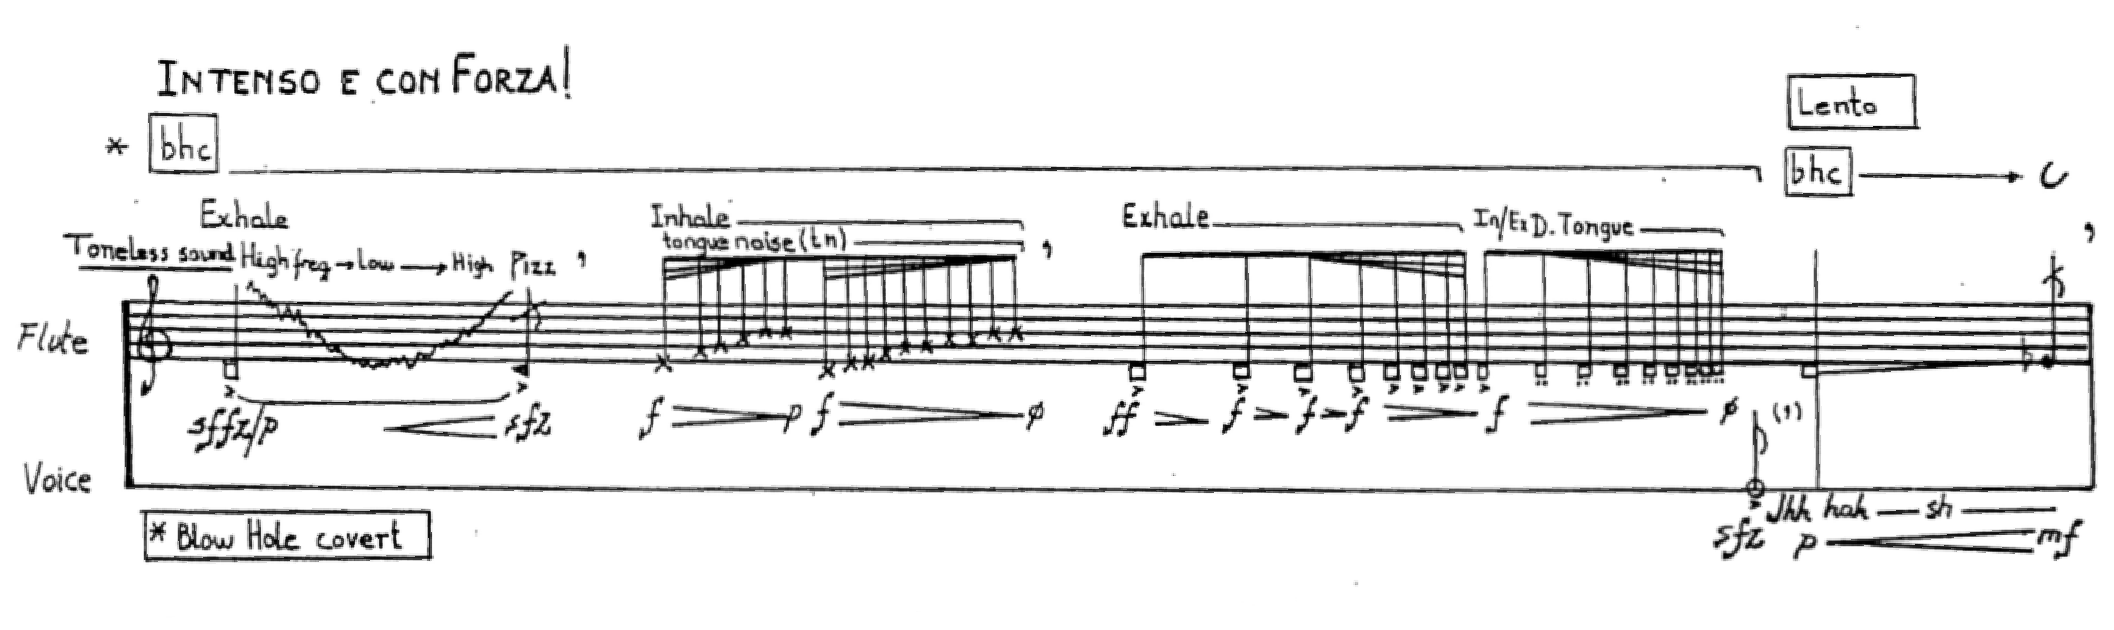
\includegraphics[width=1\textwidth]{bhc}
\caption{Notación de \textit{Blow Hole Covert} se observa en la parte superior del sistema.}
\end{center}
\end{figure}
\end{frame}

\begin{frame}{Aliento/Arrugas de Marcelo Toledo}{Notación}
\begin{figure}[H]
\begin{center}
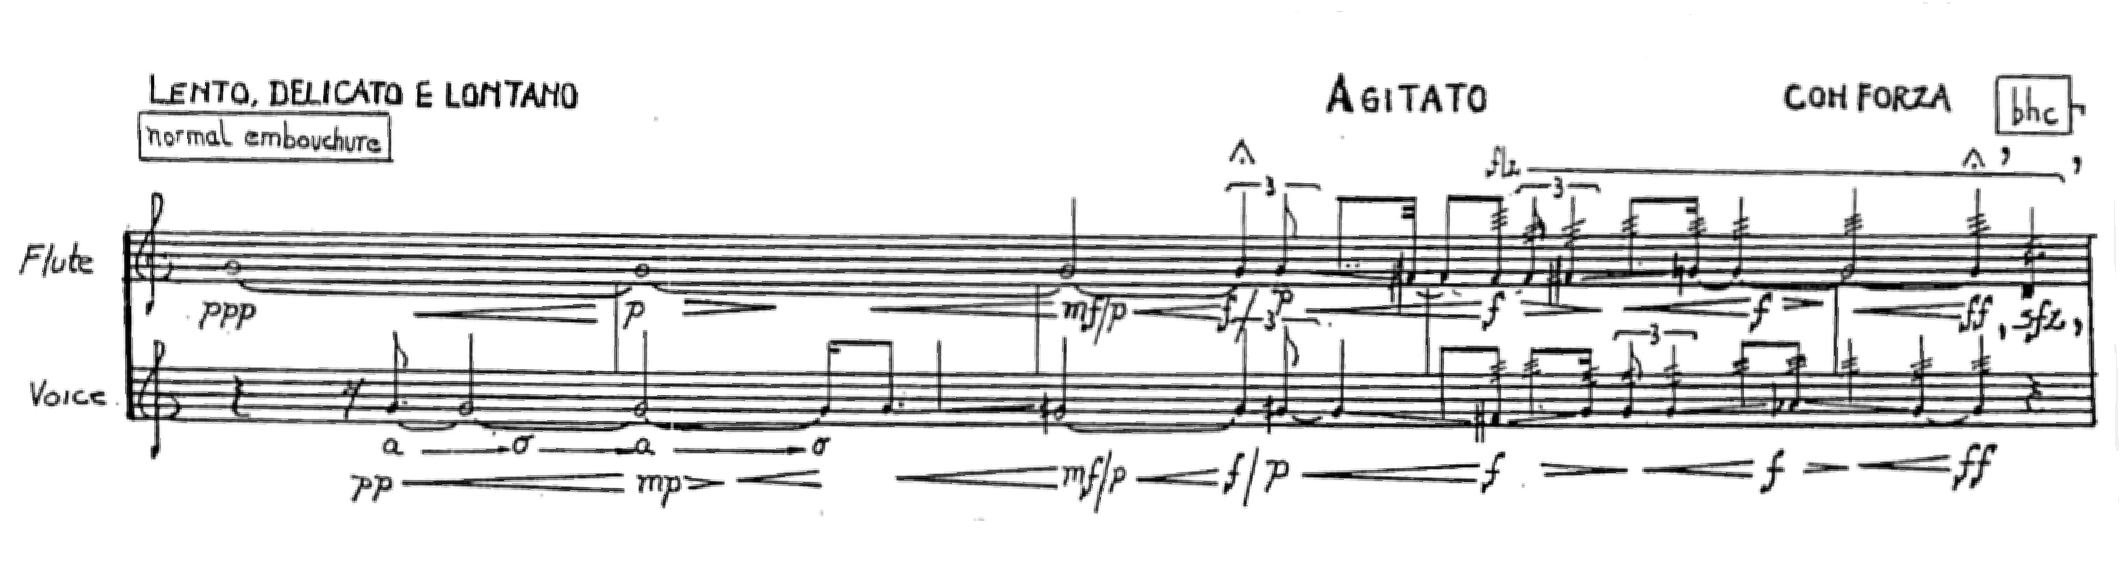
\includegraphics[width=1\textwidth]{normal} 
\caption{Notación de \textit{Normal Embouchure} se observa en la parte superior del sistema.}
\end{center}
\end{figure}
\end{frame}

\begin{frame}{Aliento/Arrugas de Marcelo Toledo}{Notación}
\begin{figure}[H]
\begin{center}
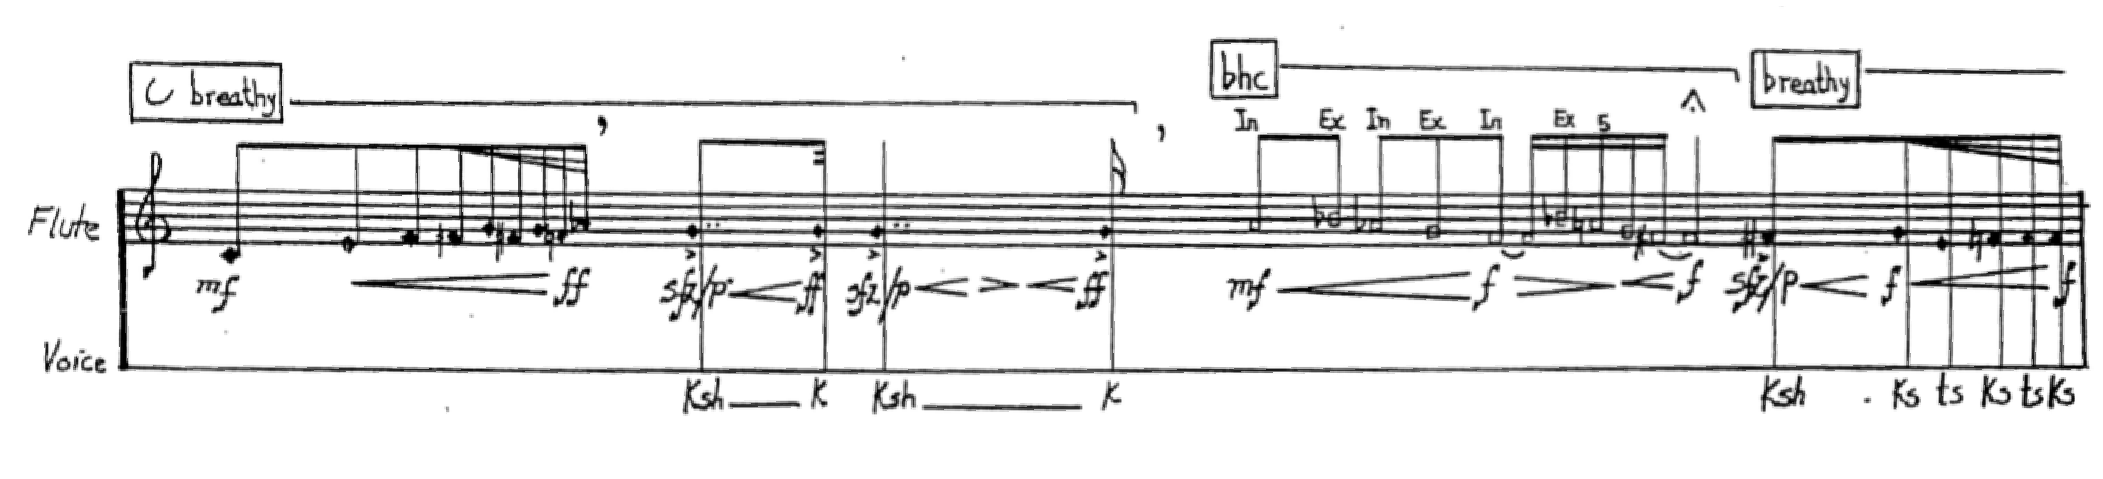
\includegraphics[width=1\textwidth]{breathy} 
\caption{Notación de \textit{Breathy Embouchure} se observa en la parte superior del sistema.}
\end{center}
\end{figure}
\end{frame}

\section{Definición del Problema}

\begin{frame}{Definición del Problema}
\begin{block}{Hipótesis central} 
Los cambios de embocadura generan variaciones en el material sonoro perceptibles de forma auditiva.
\end{block}
\begin{block}{Se propone...} 
La extracción automática del tipo de embocadura a través del análisis computacional de la obra.
\end{block}
\begin{block}{Estrategia de resolución}
Enfoque tipo \textit{Reconocimiento de Patrones}. Se procesa el audio tipo \textit{Bag of Frames} a partir del cómputo de características de audio.
\end{block}
\end{frame}

\subsection{Conjunto de Datos}

\begin{frame}{Conjunto de Datos}
\begin{block}{Grabaciones}
Se cuenta con 5 grabaciones etiquetadas manualmente de Aliento/Arrugas por los intérpretes: Ulla Suokko, Pablo Somma, Emma Resmini, Juan Pablo Quinteros y Claire Chase.
\end{block}
\begin{block}{5 \textit{folds}}
Cada obra define un conjunto de test. 
\end{block}

\begin{figure}[H]
\begin{center}
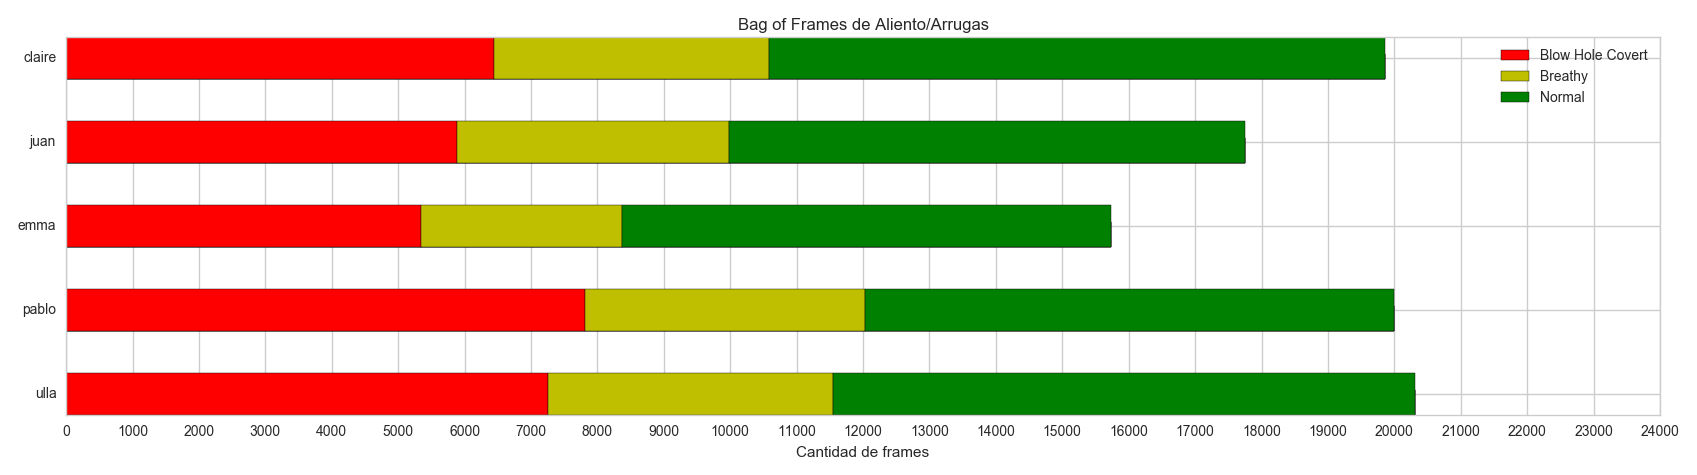
\includegraphics[width=1\textwidth]{dataset}
\end{center}
\end{figure}
\end{frame}

\subsection{Extracción de Características}

\begin{frame}{Extracción de Características}
\begin{block}{Mel-Frequency Cepstral Coefficients (MFCC)}
Extraen contenido tímbrico de la señal.
\end{block}
\begin{block}{Linear Prediction Coefficients (LPC)}
Envolvente espectral.
\end{block}
\begin{block}{Características Espectrales y Armónicas (CEA)}
\textit{Roll-off}, \textit{Centroid}, \textit{Bandwith}, \textit{Zero-Crossing Rate} y \textit{Voicing} 
\end{block}
\begin{block}{Octave-based Spectral Contrast (SC)}
Es una medida de contraste por octavas. Extrae la diferencia entre los picos y los valles.
\end{block}
\end{frame}

\section{Experimentos}

\begin{frame}{Experimentos}{Consideraciones generales}
  \begin{itemize}
  \item {
    Se utilizan tres clasificadores distintos para la evaluación de desempeño:
    \begin{itemize}
    	\item \textit{K-Nearest Neighbors} (10 vecinos)
     	\item \textit{Random Forest} (10 árboles).
     	\item \textit{Support Vector Machines} (kernel lineal).
    \end{itemize}}
  \item {   
    Se utilizan con parámetros por defecto, ya que no es objetivo del presente trabajo optimizar los clasificadores.
  }

  \end{itemize}
\end{frame}

\subsection{Primer experimento}

\begin{frame}{Primer experimento}
\begin{block}{Objetivo}
Evaluar el poder de separación de embocaduras de las características propuestas y determinar la de mejor desempeño.
\end{block}
\begin{block}{Parámetros de la extracción de características:}
\begin{itemize}
	\item Característcas Espectrales y Armónicas: (a) $11ms$ y $50\%$ de salto (256-128 muestras), (b) $23ms$ y $50\%$  (1024-512 muestras) y por último (c) $46ms$ y $50\%$  (2048-1024 muestras).
%	\begin{itemize}
%		\item Voicing: Número de retardos: 250 muestras.
%		\item Roll-off: $\lambda=85\%$
%		\item Centroid, Bandwith y Zero-Crossing Rate: quedan definidos por el largo de la ventana de análisis y el salto.
%	\end{itemize}
	\item MFCC: Ventana de análisis de $23ms$ y salto del $50\%$, 40 bandas Mel y liftrado: (a) 20 coeficientes, (b) 30 coeficientes y (c) 40 coeficientes.
	\item LPC: Ventana de análisis de $23ms$ y salto del $50\%$ y cantidad de polos: (a) 10, (b) 20 y (c) 40.
	\item SC: Ventana de análisis de $23ms$ y salto del $50\%$ y numero de bandas: (a) 3 y (b) 6.
\end{itemize}
\end{block}
\end{frame}

\begin{frame}{Primer experimento}
\begin{block}{Resultados}
\begin{figure}[H]
\begin{center}
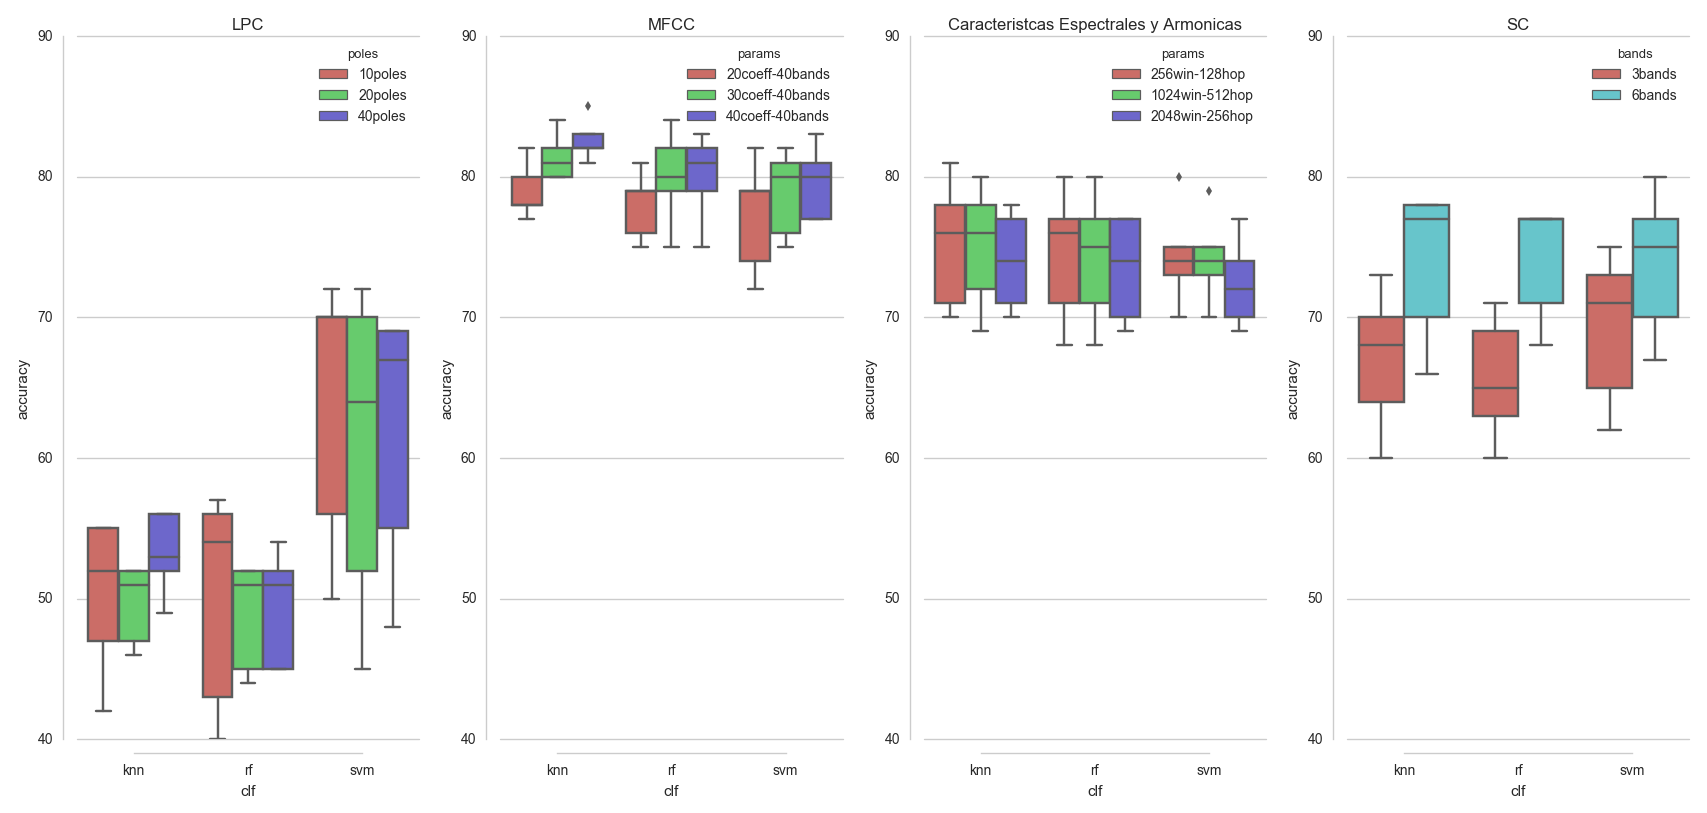
\includegraphics[width=1\textwidth]{exp1_comparacion} 
\end{center}
\end{figure}
\end{block}

\end{frame}

\begin{frame}{Primer experimento}
\begin{block}{Evaluación de resultados}
\begin{itemize}
\item \textit{LPC}: El peor desempeño. Además la variación del número de polos no muestra variaciones significativas.
\item \textit{SC}: Desempeño medio. Existe una mejora notoria al aumentar las bandas.
\item \textit{CEA}: Desempeño medio. La variación de la ventana de análisis no genera cambios apreciables. Alguna estrategia de decorrelación podría mejorar los resultados.
\item \textit{MFCC}: El mejor desempeño. Contrapartida el número de dimensiones del vector de características.
\item \textit{k-NN}: Salvo para \textit{LPC} mejor desempeño entre clasificadores.
\end{itemize}
\end{block}
\end{frame}

\begin{frame}{Primer experimento}
\begin{block}{Matrices de confusión}
\begin{figure}[H]
\begin{center}
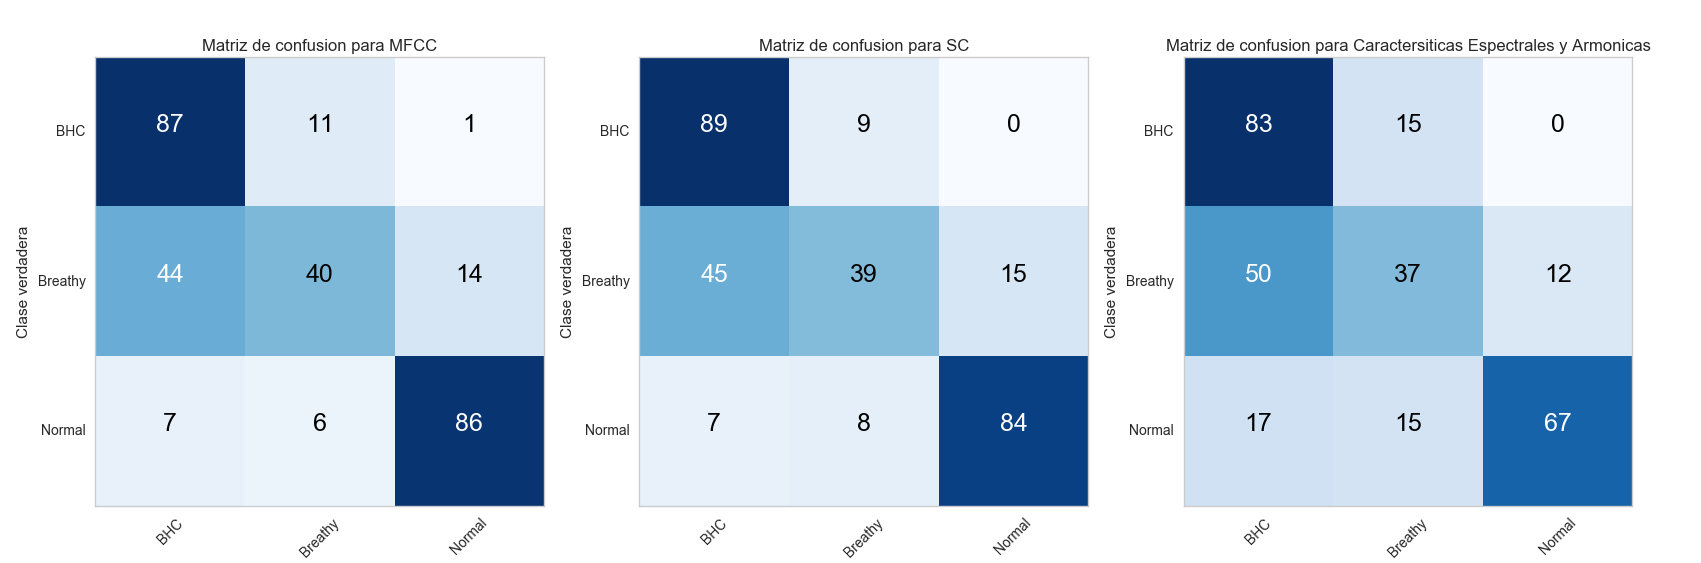
\includegraphics[width=1\textwidth]{exp1_confusion} 
\end{center}
\end{figure}
\begin{itemize}
\item Independientemente de los \textit{features} las clases \textit{Blow Hole Covert} y \textit{Normal Embouchure} se separan frente al resto.
\item \textit{Breathy} se confunde principalmente con \textit{Normal Embouchure}
\end{itemize}
\end{block}
\end{frame}


\subsection{Segundo experimento}

\begin{frame}{Segundo Experimento}
\begin{block}{Objetivo}
Evaluar el desempeño de \textit{MFCC} en un problema reducido: \textit{Blow Hole Covert} Vs. \textit{Breathy Embouchure}.
\begin{itemize}
\item Por simpleza se trabaja solamente con 40 bandas \textit{Mel} y 20 coeficientes.
\end{itemize}
\end{block}
\begin{block}{Matrices de confusión}
\begin{figure}[H]
\begin{center}
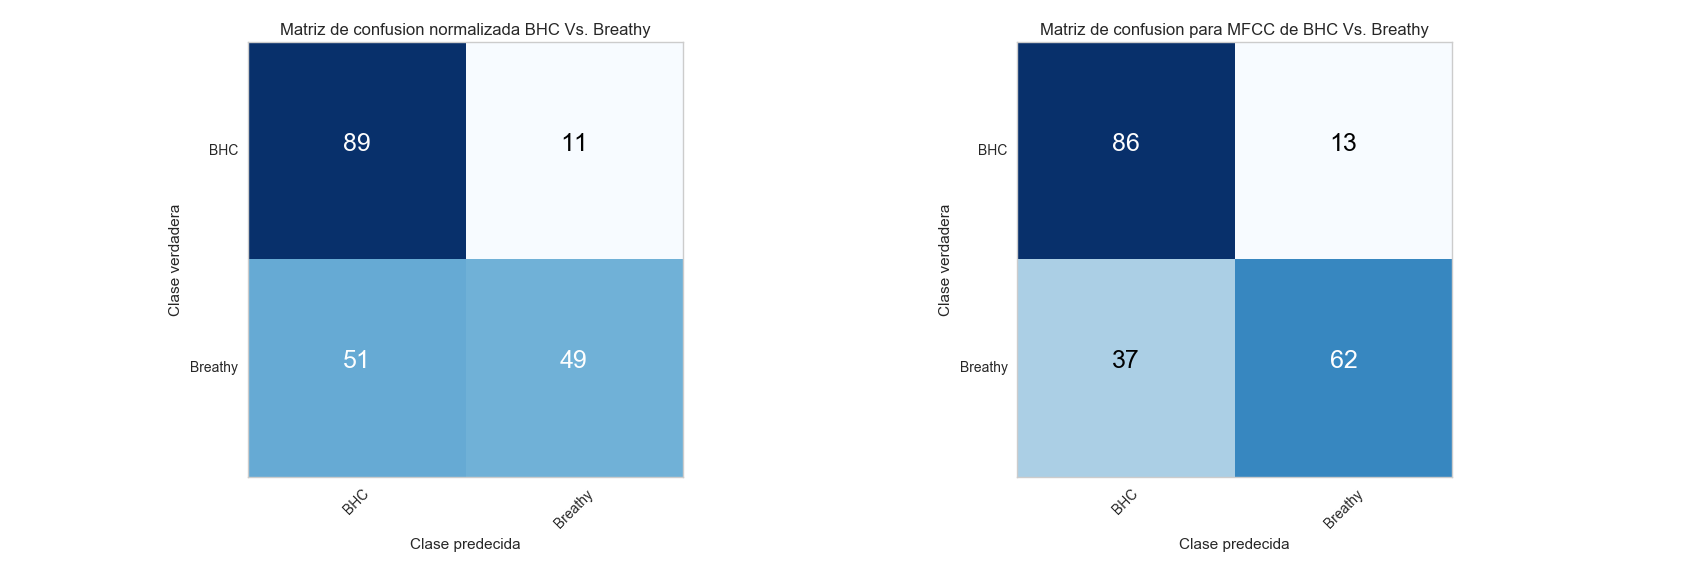
\includegraphics[width=0.9\textwidth]{exp2_confusion} 
\end{center}
\end{figure}
\end{block}
\end{frame}

\begin{frame}{Segundo Experimento}
\begin{block}{Evaluación de resultados}
\begin{itemize}
\item La confusión de \textit{Breathy} sigue siendo considerable con un $37\%$.
\item Existe una mejoría con respecto al problema de tres clases.
\item Una estrategia de clasificadores en cascada mejoraría el desempeño general, a cambio de costo computacional.
\end{itemize}
\end{block}
\end{frame}

\subsection{Refinamiento de la extracción de características basada en MFCC}

\begin{frame}{Blocks}
\begin{block}{Block Title}
You can also highlight sections of your presentation in a block, with it's own title
\end{block}
\begin{theorem}
There are separate environments for theorems, examples, definitions and proofs.
\end{theorem}
\begin{example}
Here is an example of an example block.
\end{example}
\end{frame}

\section{Conclusiones}

\begin{frame}{Blocks}
\begin{block}{Block Title}
You can also highlight sections of your presentation in a block, with it's own title
\end{block}
\begin{theorem}
There are separate environments for theorems, examples, definitions and proofs.
\end{theorem}
\begin{example}
Here is an example of an example block.
\end{example}
\end{frame}

\subsection{Trabajo a Futuro}

\begin{frame}{Blocks}
\begin{block}{Block Title}
You can also highlight sections of your presentation in a block, with it's own title
\end{block}
\begin{theorem}
There are separate environments for theorems, examples, definitions and proofs.
\end{theorem}
\begin{example}
Here is an example of an example block.
\end{example}
\end{frame}

%% Placing a * after \section means it will not show in the
%% outline or table of contents.
%\section*{Summary}
%
%\begin{frame}{Summary}
%  \begin{itemize}
%  \item
%    The \alert{first main message} of your talk in one or two lines.
%  \item
%    The \alert{second main message} of your talk in one or two lines.
%  \item
%    Perhaps a \alert{third message}, but not more than that.
%  \end{itemize}
%  
%  \begin{itemize}
%  \item
%    Outlook
%    \begin{itemize}
%    \item
%      Something you haven't solved.
%    \item
%      Something else you haven't solved.
%    \end{itemize}
%  \end{itemize}
%\end{frame}
%
%
%
% All of the following is optional and typically not needed. 
\appendix
\section<presentation>*{\appendixname}
\subsection<presentation>*{For Further Reading}

\begin{frame}[allowframebreaks]
  \frametitle<presentation>{Literatura sobre Flauta}
    
  \begin{thebibliography}{}
    
  \beamertemplatebookbibitems
  % Start with overview books.

  \bibitem{piston1955orchestration}
    A.~Author.
    \newblock {\em Handbook of Everything}.
    \newblock Some Press, 1990.
 
    
  \beamertemplatearticlebibitems
  % Followed by interesting articles. Keep the list short. 

  \bibitem{Someone2000}
    S.~Someone.
    \newblock On this and that.
    \newblock {\em Journal of This and That}, 2(1):50--100,
    2000.
  \end{thebibliography}
\end{frame}

\end{document}


